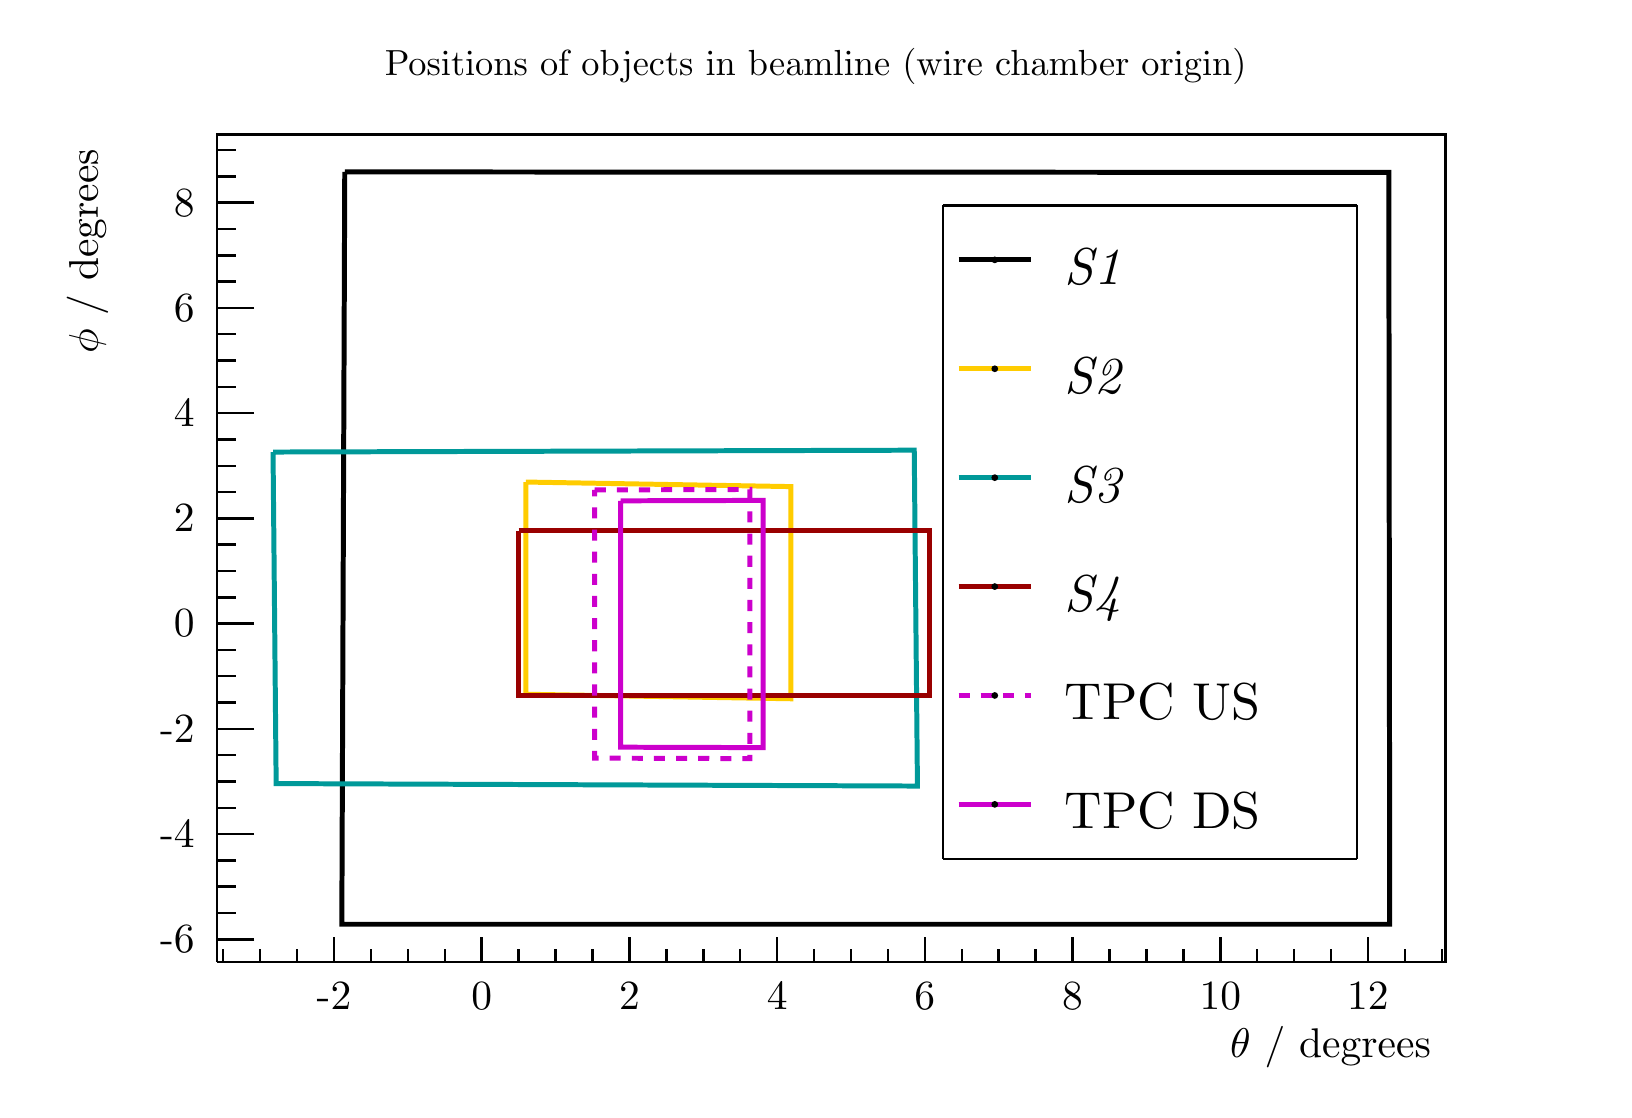
\begin{tikzpicture}
\pgfdeclareplotmark{cross} {
\pgfpathmoveto{\pgfpoint{-0.3\pgfplotmarksize}{\pgfplotmarksize}}
\pgfpathlineto{\pgfpoint{+0.3\pgfplotmarksize}{\pgfplotmarksize}}
\pgfpathlineto{\pgfpoint{+0.3\pgfplotmarksize}{0.3\pgfplotmarksize}}
\pgfpathlineto{\pgfpoint{+1\pgfplotmarksize}{0.3\pgfplotmarksize}}
\pgfpathlineto{\pgfpoint{+1\pgfplotmarksize}{-0.3\pgfplotmarksize}}
\pgfpathlineto{\pgfpoint{+0.3\pgfplotmarksize}{-0.3\pgfplotmarksize}}
\pgfpathlineto{\pgfpoint{+0.3\pgfplotmarksize}{-1.\pgfplotmarksize}}
\pgfpathlineto{\pgfpoint{-0.3\pgfplotmarksize}{-1.\pgfplotmarksize}}
\pgfpathlineto{\pgfpoint{-0.3\pgfplotmarksize}{-0.3\pgfplotmarksize}}
\pgfpathlineto{\pgfpoint{-1.\pgfplotmarksize}{-0.3\pgfplotmarksize}}
\pgfpathlineto{\pgfpoint{-1.\pgfplotmarksize}{0.3\pgfplotmarksize}}
\pgfpathlineto{\pgfpoint{-0.3\pgfplotmarksize}{0.3\pgfplotmarksize}}
\pgfpathclose
\pgfusepathqstroke
}
\pgfdeclareplotmark{cross*} {
\pgfpathmoveto{\pgfpoint{-0.3\pgfplotmarksize}{\pgfplotmarksize}}
\pgfpathlineto{\pgfpoint{+0.3\pgfplotmarksize}{\pgfplotmarksize}}
\pgfpathlineto{\pgfpoint{+0.3\pgfplotmarksize}{0.3\pgfplotmarksize}}
\pgfpathlineto{\pgfpoint{+1\pgfplotmarksize}{0.3\pgfplotmarksize}}
\pgfpathlineto{\pgfpoint{+1\pgfplotmarksize}{-0.3\pgfplotmarksize}}
\pgfpathlineto{\pgfpoint{+0.3\pgfplotmarksize}{-0.3\pgfplotmarksize}}
\pgfpathlineto{\pgfpoint{+0.3\pgfplotmarksize}{-1.\pgfplotmarksize}}
\pgfpathlineto{\pgfpoint{-0.3\pgfplotmarksize}{-1.\pgfplotmarksize}}
\pgfpathlineto{\pgfpoint{-0.3\pgfplotmarksize}{-0.3\pgfplotmarksize}}
\pgfpathlineto{\pgfpoint{-1.\pgfplotmarksize}{-0.3\pgfplotmarksize}}
\pgfpathlineto{\pgfpoint{-1.\pgfplotmarksize}{0.3\pgfplotmarksize}}
\pgfpathlineto{\pgfpoint{-0.3\pgfplotmarksize}{0.3\pgfplotmarksize}}
\pgfpathclose
\pgfusepathqfillstroke
}
\pgfdeclareplotmark{newstar} {
\pgfpathmoveto{\pgfqpoint{0pt}{\pgfplotmarksize}}
\pgfpathlineto{\pgfqpointpolar{44}{0.5\pgfplotmarksize}}
\pgfpathlineto{\pgfqpointpolar{18}{\pgfplotmarksize}}
\pgfpathlineto{\pgfqpointpolar{-20}{0.5\pgfplotmarksize}}
\pgfpathlineto{\pgfqpointpolar{-54}{\pgfplotmarksize}}
\pgfpathlineto{\pgfqpointpolar{-90}{0.5\pgfplotmarksize}}
\pgfpathlineto{\pgfqpointpolar{234}{\pgfplotmarksize}}
\pgfpathlineto{\pgfqpointpolar{198}{0.5\pgfplotmarksize}}
\pgfpathlineto{\pgfqpointpolar{162}{\pgfplotmarksize}}
\pgfpathlineto{\pgfqpointpolar{134}{0.5\pgfplotmarksize}}
\pgfpathclose
\pgfusepathqstroke
}
\pgfdeclareplotmark{newstar*} {
\pgfpathmoveto{\pgfqpoint{0pt}{\pgfplotmarksize}}
\pgfpathlineto{\pgfqpointpolar{44}{0.5\pgfplotmarksize}}
\pgfpathlineto{\pgfqpointpolar{18}{\pgfplotmarksize}}
\pgfpathlineto{\pgfqpointpolar{-20}{0.5\pgfplotmarksize}}
\pgfpathlineto{\pgfqpointpolar{-54}{\pgfplotmarksize}}
\pgfpathlineto{\pgfqpointpolar{-90}{0.5\pgfplotmarksize}}
\pgfpathlineto{\pgfqpointpolar{234}{\pgfplotmarksize}}
\pgfpathlineto{\pgfqpointpolar{198}{0.5\pgfplotmarksize}}
\pgfpathlineto{\pgfqpointpolar{162}{\pgfplotmarksize}}
\pgfpathlineto{\pgfqpointpolar{134}{0.5\pgfplotmarksize}}
\pgfpathclose
\pgfusepathqfillstroke
}
\definecolor{c}{rgb}{1,1,1};
\draw [color=c, fill=c] (0,0) rectangle (20,13.474);
\draw [color=c, fill=c] (2.4,1.61688) rectangle (18,12.1266);
\definecolor{c}{rgb}{0,0,0};
\draw [c,line width=0.9] (2.4,1.61688) -- (2.4,12.1266) -- (18,12.1266) -- (18,1.61688) -- (2.4,1.61688);
\definecolor{c}{rgb}{1,1,1};
\draw [color=c, fill=c] (2.4,1.61688) rectangle (18,12.1266);
\definecolor{c}{rgb}{0,0,0};
\draw [c,line width=0.9] (2.4,1.61688) -- (2.4,12.1266) -- (18,12.1266) -- (18,1.61688) -- (2.4,1.61688);
\draw [c,line width=0.9] (2.4,1.61688) -- (18,1.61688);
\draw [c,line width=0.9] (3.88349,1.93217) -- (3.88349,1.61688);
\draw [c,line width=0.9] (4.35247,1.77452) -- (4.35247,1.61688);
\draw [c,line width=0.9] (4.82145,1.77452) -- (4.82145,1.61688);
\draw [c,line width=0.9] (5.29044,1.77452) -- (5.29044,1.61688);
\draw [c,line width=0.9] (5.75942,1.93217) -- (5.75942,1.61688);
\draw [c,line width=0.9] (6.22841,1.77452) -- (6.22841,1.61688);
\draw [c,line width=0.9] (6.69739,1.77452) -- (6.69739,1.61688);
\draw [c,line width=0.9] (7.16638,1.77452) -- (7.16638,1.61688);
\draw [c,line width=0.9] (7.63536,1.93217) -- (7.63536,1.61688);
\draw [c,line width=0.9] (8.10435,1.77452) -- (8.10435,1.61688);
\draw [c,line width=0.9] (8.57333,1.77452) -- (8.57333,1.61688);
\draw [c,line width=0.9] (9.04231,1.77452) -- (9.04231,1.61688);
\draw [c,line width=0.9] (9.5113,1.93217) -- (9.5113,1.61688);
\draw [c,line width=0.9] (9.98028,1.77452) -- (9.98028,1.61688);
\draw [c,line width=0.9] (10.4493,1.77452) -- (10.4493,1.61688);
\draw [c,line width=0.9] (10.9183,1.77452) -- (10.9183,1.61688);
\draw [c,line width=0.9] (11.3872,1.93217) -- (11.3872,1.61688);
\draw [c,line width=0.9] (11.8562,1.77452) -- (11.8562,1.61688);
\draw [c,line width=0.9] (12.3252,1.77452) -- (12.3252,1.61688);
\draw [c,line width=0.9] (12.7942,1.77452) -- (12.7942,1.61688);
\draw [c,line width=0.9] (13.2632,1.93217) -- (13.2632,1.61688);
\draw [c,line width=0.9] (13.7322,1.77452) -- (13.7322,1.61688);
\draw [c,line width=0.9] (14.2011,1.77452) -- (14.2011,1.61688);
\draw [c,line width=0.9] (14.6701,1.77452) -- (14.6701,1.61688);
\draw [c,line width=0.9] (15.1391,1.93217) -- (15.1391,1.61688);
\draw [c,line width=0.9] (15.6081,1.77452) -- (15.6081,1.61688);
\draw [c,line width=0.9] (16.0771,1.77452) -- (16.0771,1.61688);
\draw [c,line width=0.9] (16.5461,1.77452) -- (16.5461,1.61688);
\draw [c,line width=0.9] (17.015,1.93217) -- (17.015,1.61688);
\draw [c,line width=0.9] (3.88349,1.93217) -- (3.88349,1.61688);
\draw [c,line width=0.9] (3.4145,1.77452) -- (3.4145,1.61688);
\draw [c,line width=0.9] (2.94552,1.77452) -- (2.94552,1.61688);
\draw [c,line width=0.9] (2.47653,1.77452) -- (2.47653,1.61688);
\draw [c,line width=0.9] (17.015,1.93217) -- (17.015,1.61688);
\draw [c,line width=0.9] (17.484,1.77452) -- (17.484,1.61688);
\draw [c,line width=0.9] (17.953,1.77452) -- (17.953,1.61688);
\draw [anchor=base] (3.88349,1.01055) node[scale=1.49939, color=c, rotate=0]{-2};
\draw [anchor=base] (5.75942,1.01055) node[scale=1.49939, color=c, rotate=0]{0};
\draw [anchor=base] (7.63536,1.01055) node[scale=1.49939, color=c, rotate=0]{2};
\draw [anchor=base] (9.5113,1.01055) node[scale=1.49939, color=c, rotate=0]{4};
\draw [anchor=base] (11.3872,1.01055) node[scale=1.49939, color=c, rotate=0]{6};
\draw [anchor=base] (13.2632,1.01055) node[scale=1.49939, color=c, rotate=0]{8};
\draw [anchor=base] (15.1391,1.01055) node[scale=1.49939, color=c, rotate=0]{10};
\draw [anchor=base] (17.015,1.01055) node[scale=1.49939, color=c, rotate=0]{12};
\draw [anchor= east] (18,0.538959) node[scale=1.49939, color=c, rotate=0]{$\theta$ / degrees};
\draw [c,line width=0.9] (2.4,1.61688) -- (2.4,12.1266);
\draw [c,line width=0.9] (2.868,1.90318) -- (2.4,1.90318);
\draw [c,line width=0.9] (2.634,2.2373) -- (2.4,2.2373);
\draw [c,line width=0.9] (2.634,2.57142) -- (2.4,2.57142);
\draw [c,line width=0.9] (2.634,2.90555) -- (2.4,2.90555);
\draw [c,line width=0.9] (2.868,3.23967) -- (2.4,3.23967);
\draw [c,line width=0.9] (2.634,3.57379) -- (2.4,3.57379);
\draw [c,line width=0.9] (2.634,3.90792) -- (2.4,3.90792);
\draw [c,line width=0.9] (2.634,4.24204) -- (2.4,4.24204);
\draw [c,line width=0.9] (2.868,4.57616) -- (2.4,4.57616);
\draw [c,line width=0.9] (2.634,4.91028) -- (2.4,4.91028);
\draw [c,line width=0.9] (2.634,5.24441) -- (2.4,5.24441);
\draw [c,line width=0.9] (2.634,5.57853) -- (2.4,5.57853);
\draw [c,line width=0.9] (2.868,5.91265) -- (2.4,5.91265);
\draw [c,line width=0.9] (2.634,6.24678) -- (2.4,6.24678);
\draw [c,line width=0.9] (2.634,6.5809) -- (2.4,6.5809);
\draw [c,line width=0.9] (2.634,6.91502) -- (2.4,6.91502);
\draw [c,line width=0.9] (2.868,7.24915) -- (2.4,7.24915);
\draw [c,line width=0.9] (2.634,7.58327) -- (2.4,7.58327);
\draw [c,line width=0.9] (2.634,7.91739) -- (2.4,7.91739);
\draw [c,line width=0.9] (2.634,8.25151) -- (2.4,8.25151);
\draw [c,line width=0.9] (2.868,8.58564) -- (2.4,8.58564);
\draw [c,line width=0.9] (2.634,8.91976) -- (2.4,8.91976);
\draw [c,line width=0.9] (2.634,9.25388) -- (2.4,9.25388);
\draw [c,line width=0.9] (2.634,9.58801) -- (2.4,9.58801);
\draw [c,line width=0.9] (2.868,9.92213) -- (2.4,9.92213);
\draw [c,line width=0.9] (2.634,10.2563) -- (2.4,10.2563);
\draw [c,line width=0.9] (2.634,10.5904) -- (2.4,10.5904);
\draw [c,line width=0.9] (2.634,10.9245) -- (2.4,10.9245);
\draw [c,line width=0.9] (2.868,11.2586) -- (2.4,11.2586);
\draw [c,line width=0.9] (2.868,1.90318) -- (2.4,1.90318);
\draw [c,line width=0.9] (2.868,11.2586) -- (2.4,11.2586);
\draw [c,line width=0.9] (2.634,11.5927) -- (2.4,11.5927);
\draw [c,line width=0.9] (2.634,11.9269) -- (2.4,11.9269);
\draw [anchor= east] (2.3,1.90318) node[scale=1.49939, color=c, rotate=0]{-6};
\draw [anchor= east] (2.3,3.23967) node[scale=1.49939, color=c, rotate=0]{-4};
\draw [anchor= east] (2.3,4.57616) node[scale=1.49939, color=c, rotate=0]{-2};
\draw [anchor= east] (2.3,5.91265) node[scale=1.49939, color=c, rotate=0]{0};
\draw [anchor= east] (2.3,7.24915) node[scale=1.49939, color=c, rotate=0]{2};
\draw [anchor= east] (2.3,8.58564) node[scale=1.49939, color=c, rotate=0]{4};
\draw [anchor= east] (2.3,9.92213) node[scale=1.49939, color=c, rotate=0]{6};
\draw [anchor= east] (2.3,11.2586) node[scale=1.49939, color=c, rotate=0]{8};
\draw [anchor= east] (0.753024,12.1266) node[scale=1.49939, color=c, rotate=90]{$\phi$ / degrees};
\draw [c,line width=1.8] (4.02001,11.6489) -- (17.2792,11.643) -- (17.2909,2.09459) -- (3.98258,2.09459) -- (4.02001,11.6489);
\definecolor{c}{rgb}{1,0.8,0};
\draw [c,line width=1.8] (6.32024,7.71036) -- (6.32024,5.01555) -- (9.6851,4.95805) -- (9.6851,7.65257) -- (6.32024,7.71036);
\definecolor{c}{rgb}{0,0.6,0.6};
\draw [c,line width=1.8] (3.10909,8.09147) -- (11.2523,8.11493) -- (11.293,3.84961) -- (3.14872,3.88101) -- (3.10909,8.09147);
\definecolor{c}{rgb}{0.6,0,0};
\draw [c,line width=1.8] (6.22774,7.09184) -- (11.4508,7.09184) -- (11.4508,4.99824) -- (6.22774,4.99824) -- (6.22774,7.09184);
\definecolor{c}{rgb}{0.8,0,0.8};
\draw [c,dash pattern=on 4.00pt off 4.00pt ,line width=1.8] (7.19412,7.60986) -- (9.16463,7.61621) -- (9.16463,4.19793) -- (7.19412,4.20431) -- (7.19412,7.60986);
\draw [c,line width=1.8] (7.52371,7.47197) -- (9.33375,7.47732) -- (9.33375,4.33772) -- (7.52371,4.34311) -- (7.52371,7.47197);
\definecolor{c}{rgb}{0,0,0};
\draw (10,12.9947) node[scale=1.31197, color=c, rotate=0]{Positions of objects in beamline (wire chamber origin)};
\definecolor{c}{rgb}{1,1,1};
\draw [color=c, fill=c] (11.6174,2.92546) rectangle (16.8776,11.2236);
\definecolor{c}{rgb}{0,0,0};
\draw [c,line width=0.9] (11.6174,2.92546) -- (16.8776,2.92546);
\draw [c,line width=0.9] (16.8776,2.92546) -- (16.8776,11.2236);
\draw [c,line width=0.9] (16.8776,11.2236) -- (11.6174,11.2236);
\draw [c,line width=0.9] (11.6174,11.2236) -- (11.6174,2.92546);
\draw [anchor=base west] (12.9325,10.2209) node[scale=1.87424, color=c, rotate=0]{$\mathit{S1}$};
\definecolor{c}{rgb}{1,1,1};
\draw [c, fill=c] (11.8147,10.0481) -- (12.7352,10.0481) -- (12.7352,11.0162) -- (11.8147,11.0162);
\definecolor{c}{rgb}{0,0,0};
\draw [c,line width=1.8] (11.8147,10.5321) -- (12.7352,10.5321);
\foreach \P in {(12.275,10.5321)}{\draw[mark options={color=c,fill=c},mark size=2.402402pt,mark=*,mark size=1pt] plot coordinates {\P};}
\draw [anchor=base west] (12.9325,8.8379) node[scale=1.87424, color=c, rotate=0]{$\mathit{S2}$};
\definecolor{c}{rgb}{1,1,1};
\draw [c, fill=c] (11.8147,8.66503) -- (12.7352,8.66503) -- (12.7352,9.63315) -- (11.8147,9.63315);
\definecolor{c}{rgb}{1,0.8,0};
\draw [c,line width=1.8] (11.8147,9.14909) -- (12.7352,9.14909);
\definecolor{c}{rgb}{0,0,0};
\foreach \P in {(12.275,9.14909)}{\draw[mark options={color=c,fill=c},mark size=2.402402pt,mark=*,mark size=1pt] plot coordinates {\P};}
\draw [anchor=base west] (12.9325,7.45488) node[scale=1.87424, color=c, rotate=0]{$\mathit{S3}$};
\definecolor{c}{rgb}{1,1,1};
\draw [c, fill=c] (11.8147,7.282) -- (12.7352,7.282) -- (12.7352,8.25012) -- (11.8147,8.25012);
\definecolor{c}{rgb}{0,0.6,0.6};
\draw [c,line width=1.8] (11.8147,7.76606) -- (12.7352,7.76606);
\definecolor{c}{rgb}{0,0,0};
\foreach \P in {(12.275,7.76606)}{\draw[mark options={color=c,fill=c},mark size=2.402402pt,mark=*,mark size=1pt] plot coordinates {\P};}
\draw [anchor=base west] (12.9325,6.07185) node[scale=1.87424, color=c, rotate=0]{$\mathit{S4}$};
\definecolor{c}{rgb}{1,1,1};
\draw [c, fill=c] (11.8147,5.89897) -- (12.7352,5.89897) -- (12.7352,6.86709) -- (11.8147,6.86709);
\definecolor{c}{rgb}{0.6,0,0};
\draw [c,line width=1.8] (11.8147,6.38303) -- (12.7352,6.38303);
\definecolor{c}{rgb}{0,0,0};
\foreach \P in {(12.275,6.38303)}{\draw[mark options={color=c,fill=c},mark size=2.402402pt,mark=*,mark size=1pt] plot coordinates {\P};}
\draw [anchor=base west] (12.9325,4.68882) node[scale=1.87424, color=c, rotate=0]{TPC US};
\definecolor{c}{rgb}{1,1,1};
\draw [c, fill=c] (11.8147,4.51594) -- (12.7352,4.51594) -- (12.7352,5.48406) -- (11.8147,5.48406);
\definecolor{c}{rgb}{0.8,0,0.8};
\draw [c,dash pattern=on 4.00pt off 4.00pt ,line width=1.8] (11.8147,5) -- (12.7352,5);
\definecolor{c}{rgb}{0,0,0};
\foreach \P in {(12.275,5)}{\draw[mark options={color=c,fill=c},mark size=2.402402pt,mark=*,mark size=1pt] plot coordinates {\P};}
\draw [anchor=base west] (12.9325,3.30579) node[scale=1.87424, color=c, rotate=0]{TPC DS};
\definecolor{c}{rgb}{1,1,1};
\draw [c, fill=c] (11.8147,3.13291) -- (12.7352,3.13291) -- (12.7352,4.10103) -- (11.8147,4.10103);
\definecolor{c}{rgb}{0.8,0,0.8};
\draw [c,line width=1.8] (11.8147,3.61697) -- (12.7352,3.61697);
\definecolor{c}{rgb}{0,0,0};
\foreach \P in {(12.275,3.61697)}{\draw[mark options={color=c,fill=c},mark size=2.402402pt,mark=*,mark size=1pt] plot coordinates {\P};}
\end{tikzpicture}
